\begin{frame}{Ejemplo: Mundo de una aspiradora}
    \begin{columns}
      \begin{column}{0.6\textwidth}
        \emphblue{Estado-\'Unico}, comienza en \#5.
        \textcolor{red}{Solución ??}\\
        \textcolor{Pink}{$[Derecha, Aspirar]$}\\~\\
       
        \emphblue{Conformado}, comienza en
        \textcolor{Pink}{$\{1,2,3,4,5,6,7,8\}$} e.g., \textcolor{Pink}{Derecha} va a \textcolor{Pink}{$\{2,4,6,8\}$}
        \textcolor{red}{Solución ??}\\
        \textcolor{Pink}{$[Derecha, Aspirar, Izquierda, Aspirar]$}\\~\\
        
        \emphblue{Contingencia}, comienza en \#5.\\
        Ley de Murphy: \textcolor{Pink}{Aspirar} puede ensuciar una alfombra l\'impia.\\
        Detecci\'on local: suciedad, s\'olo por locaci\'on.
        \textcolor{red}{Soluci\'on ??}\\
        
        \end{column}
      \begin{column}{0.4\textwidth}
      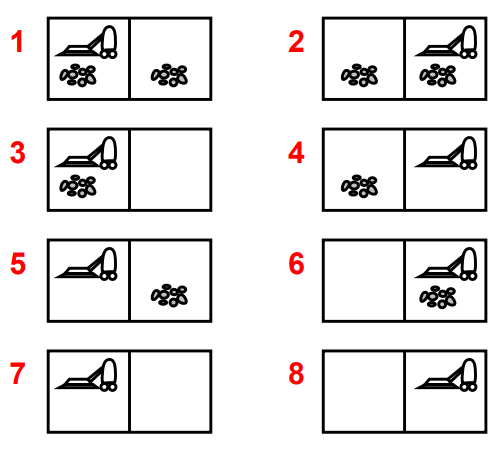
\includegraphics[width=0.8\textwidth]{9_image_example1.PNG}
      \end{column}
    \end{columns}

    
\end{frame}
